% Created 2023-04-06 czw 16:08
% Intended LaTeX compiler: pdflatex
\documentclass[11pt]{article}
\usepackage[utf8]{inputenc}
\usepackage[T1]{fontenc}
\usepackage{graphicx}
\usepackage{grffile}
\usepackage{longtable}
\usepackage{wrapfig}
\usepackage{rotating}
\usepackage[normalem]{ulem}
\usepackage{amsmath}
\usepackage{textcomp}
\usepackage{amssymb}
\usepackage{capt-of}
\usepackage{hyperref}
\usepackage{polski}
\usepackage{indentfirst}
% do bibliografii
\usepackage[sorting=ydnt, backend=biber]{biblatex}
\usepackage{tabularx}

\usepackage[left=1.0cm,right=1.0cm,top=1.0cm,bottom=2.0cm]{geometry}

\usepackage{helvet}

\usepackage{setspace}
\usepackage{listings}
\usepackage{cleveref} % \cref    -> lepsze od \ref ???
% \usepackage{cite}     % bibliografia i \cite{}
\usepackage{xcolor}   % kolory w lstlisting
\usepackage{amssymb}  % żeby działało \mmathbb
% \usepackage{fontspec} % Arial
\usepackage[linesnumbered,ruled,vlined]{algorithm2e} % fajne algorytmy
\usepackage{etoolbox} % BeforeBeginEnvironment, AfterEndEnvironment





\lstdefinestyle{shared} {
	numbers=left,
	numbersep=1em,
	numberstyle=\tiny\color{red}\noaccsupp,
	frame=single,
	framesep=\fboxsep,
	framerule=\fboxrule,
	rulecolor=\color{red},
	xleftmargin=\dimexpr\fboxsep+\fboxrule\relax,
	xrightmargin=\dimexpr\fboxsep+\fboxrule\relax,
	breaklines=true,
	tabsize=2,
	columns=flexible,
}

\lstdefinestyle{xml} {
	style=shared,
	language={sql},
	%alsolanguage={PSTricks},
	basicstyle=\small\tt,
	keywordstyle=\color{blue},
	commentstyle=\color[rgb]{0.13,0.54,0.13},
	backgroundcolor=\color{yellow!10},
	morekeywords={
		graphicspath,
		includegraphics,
		blinddocument,
	},
}

\lstdefinestyle{pseudocode} {
	style=shared,
	language={sql},
	%alsolanguage={[Sharp]C},
	basicstyle=\small\tt,
	keywordstyle=\color{blue},
	commentstyle=\color[rgb]{0.13,0.54,0.13},
	backgroundcolor=\color{cyan!10},
	morekeywords={
		Console,
		WriteLine,
		int,
	},
}

\lstnewenvironment{xml}
{\lstset{style=xml}}
{}

\lstnewenvironment{pseudocode}
{\lstset{style=pseudocode}}
{}



\lstset{
	basicstyle=\ttfamily,
	numbers=left,
	stepnumber=1,
	showstringspaces=false,
	tabsize=1,
	breaklines=true,
	breakatwhitespace=false,
	frame=single,
	captionpos=b,
}

\setlength{\belowcaptionskip}{2pt}
\setlength{\abovecaptionskip}{2pt}
\BeforeBeginEnvironment{figure}{\vskip+12pt}
\AfterEndEnvironment{figure}{\vskip+0pt}
\BeforeBeginEnvironment{lstlisting}{\vskip+20pt}
\BeforeBeginEnvironment{table}{\vskip+15pt}







% \addbibresource{bib.bib}
% do tabel
\usepackage{float}
\usepackage{array}
\newcolumntype{P}[1]{>{\centering\arraybackslash}p{#1}}
% numerowanie obrazkow
\numberwithin{figure}{subsection}

\author{Marek Zalewski
}
\date{\today}
\title{%
	Raport z wykonanego laboratorium z optymalizacji bazy danych
}
\hypersetup{
  pdfauthor={Marek Zalewski},
  pdftitle={Raport z wykonanego laboratorium z optymalizacji bazy danych},
  pdfkeywords={},
  pdfsubject={},
  pdflang={Polish}}
\begin{document}

\maketitle
\tableofcontents

\newpage

\section{Struktura bazy danych}
	Cały kod bazy danych i zapytań znajduje się w repozytorium:
	\url{https://github.com/Drwalin/studies-mag1-OBD}
	\\
	Baza danych opisuje historię transakcji przedmiotów pomiędzy bytami w
	świecie gry, a także zmianę ich położenia. Postać gracza jest przykładowym
	bytem.
	\begin{figure}[H]
		\centering
		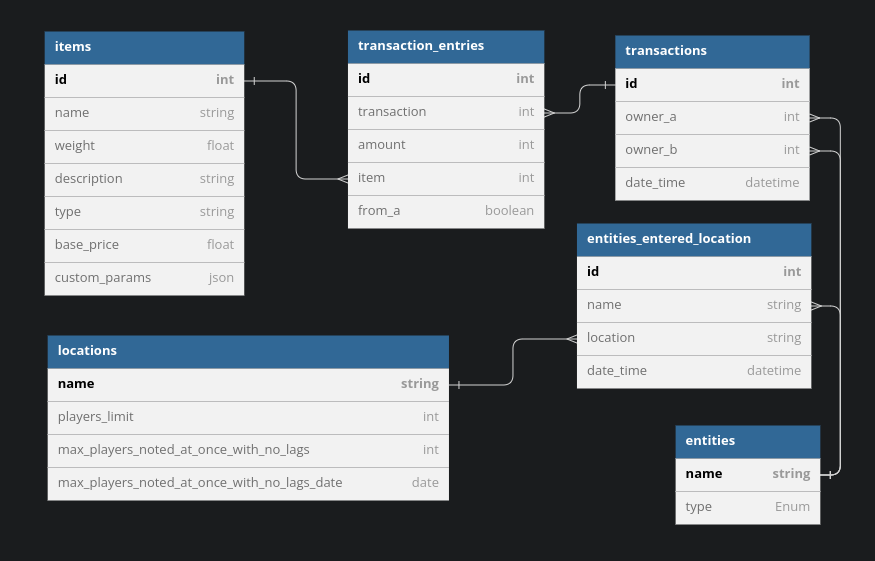
\includegraphics[width=1.0\textwidth]{./images/struktura-bazy-danych.png}
		\caption[Schemat filtra]{Struktura niezoptymalizowanej bazy danych}
		\label{fig:schemat_filtra}
	\end{figure}
	
	\begin{lstlisting}[caption={Kod utworzenia tabeli entities},captionpos=b]
CREATE TABLE entities (
	name VARCHAR(64) PRIMARY KEY NOT NULL,
	-- player, npc, mob, chest, marketplace, boss
	type VARCHAR(64) NOT NULL
);
    \end{lstlisting}

	\begin{lstlisting}[caption={Kod utworzenia tabeli items},captionpos=b]
CREATE TABLE items (
	id INT GENERATED BY DEFAULT ON NULL AS IDENTITY PRIMARY KEY,
	name VARCHAR(256) NOT NULL,
	weight FLOAT NOT NULL,
	description VARCHAR(1024),
	category VARCHAR(32) NOT NULL,
	base_price DECIMAL(11,2),
	custom_params JSON
);
    \end{lstlisting}

	\begin{lstlisting}[caption={Kod utworzenia tabeli transactions},captionpos=b]
CREATE TABLE transactions (
	id INT GENERATED BY DEFAULT ON NULL AS IDENTITY PRIMARY KEY,
	stamp TIMESTAMP NOT NULL,
	owner_a VARCHAR(64),
	owner_b VARCHAR(64),
	
	CONSTRAINT owner_a_ref
		FOREIGN KEY (owner_a)
		REFERENCES entities (name),
	CONSTRAINT owner_b_ref
		FOREIGN KEY (owner_b)
		REFERENCES entities (name)
);
    \end{lstlisting}

	\begin{lstlisting}[caption={Kod utworzenia tabeli transaction\_entries},captionpos=b]
CREATE TABLE transaction_entries (
	id INT GENERATED BY DEFAULT ON NULL AS IDENTITY PRIMARY KEY,
	transaction INT NOT NULL,
	item INT NOT NULL,
	from_a CHAR CHECK (from_a IN (0,1)),
	
	CONSTRAINT transaction_ref
		FOREIGN KEY (transaction)
		REFERENCES transactions (id),
	CONSTRAINT item_ref
		FOREIGN KEY (item)
		REFERENCES items (id)
);
    \end{lstlisting}

	\begin{lstlisting}[caption={Kod utworzenia tabeli locations},captionpos=b]
CREATE TABLE locations (
	name VARCHAR(128) NOT NULL PRIMARY KEY,
	players_limit INT NOT NULL,
	max_players_noted_at_once_with_no_lags INT,
	max_players_noted_at_once_with_no_lags_date DATE
);
    \end{lstlisting}

	\begin{lstlisting}[caption={Kod utworzenia tabeli entities\_entered\_location},captionpos=b]
CREATE TABLE entities_entered_location (
	id INT GENERATED BY DEFAULT ON NULL AS IDENTITY PRIMARY KEY,
	name VARCHAR(64) NOT NULL, -- references entities.name
	location VARCHAR(128) NOT NULL, -- references locations.name
	date_time TIMESTAMP,
	
	CONSTRAINT location_ref
		FOREIGN KEY (location)
		REFERENCES locations (name),
	CONSTRAINT entity_ref
		FOREIGN KEY (name)
		REFERENCES entities (name)
);
    \end{lstlisting}


	
\section{Funkcje, procedury i typy pomocnicze}
	Poniżej znajduje się wiele pomocniczych funkcji i procedur, które okazały
	się przydatne podczas generowania danych. 
	
	\begin{lstlisting}[caption={Pomocnicze typy},captionpos=b]
CREATE OR REPLACE TYPE t_strings AS TABLE OF VARCHAR2(1024);
CREATE OR REPLACE TYPE t_ints AS TABLE OF INT;
    \end{lstlisting}
	
	\begin{lstlisting}[caption={Funkcje pomocnicze w manipulacji czasu},captionpos=b]
CREATE OR REPLACE FUNCTION AdvanceTimestamp(
		entityName IN VARCHAR2,
		created OUT TIMESTAMP,
		lastEntry OUT TIMESTAMP) RETURN TIMESTAMP IS
BEGIN
	SELECT date_time INTO created FROM entities_entered_location E1
		WHERE name = entityName AND (
			SELECT count(*) FROM entities_entered_location E2
			WHERE name = entityName AND E1.date_time > E2.date_time
		) = 0;
	SELECT date_time INTO lastEntry FROM entities_entered_location E1
		WHERE name = entityName AND (
			SELECT count(*) FROM entities_entered_location E2
			WHERE name = entityName AND E1.date_time < E2.date_time
		) = 0;
END;

CREATE OR REPLACE FUNCTION AdvanceTimestamp(
		currentTime TIMESTAMP,
		hours_min IN NUMBER,
		hours_max IN NUMBER) RETURN TIMESTAMP IS
BEGIN
	RETURN currentTime + dbms_random.value(hours_min, hours_max) * INTERVAL '1' HOUR;
END;


CREATE OR REPLACE FUNCTION GetRandomTimestampBetween(
		t1 IN TIMESTAMP,
		t2 IN TIMESTAMP) RETURN TIMESTAMP AS
	t TIMESTAMP;
BEGIN
	SELECT t1 + dbms_random.value(0, 1) * (t2-t1)
		INTO t
		FROM dual;
	RETURN t;
END;

CREATE OR REPLACE FUNCTION GetDateOfNewestTransaction RETURN TIMESTAMP IS
	ret TIMESTAMP;
BEGIN
	SELECT stamp INTO ret FROM transactions
		ORDER BY stamp DESC FETCH FIRST 1 ROWS ONLY;
	RETURN ret;
END;
    \end{lstlisting}
	
	\begin{lstlisting}[caption={Funkcja zwracająca losową wartość krzywej
	dzwonowej},captionpos=b]
CREATE OR REPLACE FUNCTION RandomGaussian(
		minx IN NUMBER,
		maxx IN NUMBER) RETURN NUMBER AS
BEGIN
	RETURN dbms_random.value(minx/3, maxx/3)
		+ dbms_random.value(minx/3, maxx/3)
		+ dbms_random.value(minx/3, maxx/3);
END;
    \end{lstlisting}
	
	\begin{lstlisting}[caption={Pomocnicze funkcje generujące losowe ciągi
	znaków},captionpos=b]
CREATE OR REPLACE FUNCTION RandomChar(
		p_Characters IN VARCHAR2) RETURN VARCHAR2 IS
	l_res VARCHAR2(256);
	vvvv NUMBER;
BEGIN
	vvvv := round(dbms_random.value(0, length(p_Characters)-1));
	RETURN SUBSTR(p_Characters, vvvv, 1);
END;


CREATE OR REPLACE FUNCTION RandomString(
		p_Characters IN VARCHAR2,
		p_length IN NUMBER) RETURN VARCHAR2 IS
	l_res VARCHAR2(256);
BEGIN
	FOR i in 1..p_length LOOP
		l_res := l_res || RandomChar(p_Characters);
	END LOOP;
	RETURN l_res;
END;
    \end{lstlisting}
	
	\begin{lstlisting}[caption={Pomocnicze funkcje generujące losowe nazwy dla
	entity składające się z imion i nazwisk z wczytanych danych z pliku csv},
	captionpos=b]
CREATE OR REPLACE FUNCTION GenerateRandomName(
		min_chars IN NUMBER,
		max_chars IN NUMBER) RETURN VARCHAR2 IS
	value_ret VARCHAR2(1024);
	chars_count NUMBER;
	vvvv NUMBER;
BEGIN
	chars_count := dbms_random.value(min_chars, max_chars);
	value_ret := RandomChar('QWERTYUIOPASDFGHJKLZXCVBNMEYUIOA');
		
	FOR i in 1..chars_count/2 LOOP
		value_ret := value_ret || RandomChar(
			'qwertyuiopasdfghjklzxcvbnm');
		value_ret := value_ret || RandomChar(
			'qwertyuiopasdfghjklzxcvbnmaeoiuyaeoiuyae\
oiuyaeoiuyaeoiuyaeoiuyaeoiuy');
	END LOOP;
	return value_ret;
END;


CREATE OR REPLACE FUNCTION SelectRandomName RETURN VARCHAR2 IS
	v VARCHAR2(64);
BEGIN
	SELECT first_name INTO v
	FROM imported_first_names
	ORDER BY dbms_random.random FETCH FIRST 1 ROWS ONLY;
	return v;
END;

CREATE OR REPLACE FUNCTION SelectRandomLastName RETURN VARCHAR2 IS
	v VARCHAR2(64);
BEGIN
	SELECT last_name INTO v
	FROM imported_last_names
	ORDER BY dbms_random.random FETCH FIRST 1 ROWS ONLY;
	return v;
END;

CREATE OR REPLACE FUNCTION GenerateRandomEntityName RETURN VARCHAR2 IS
	value_ret VARCHAR2(1024);
	names_count NUMBER;
	last_names_count NUMBER;
BEGIN
	
	names_count := round(dbms_random.value(1, 4));
	last_names_count := round(dbms_random.value(0, 2));
	
	value_ret := SelectRandomName();
	
	FOR i in 2..names_count LOOP
		value_ret := value_ret || ' ' || SelectRandomName();
	END LOOP;
	
	FOR i in 2..last_names_count LOOP
		value_ret := value_ret || ' ' || SelectRandomLastName();
	END LOOP;
	
	return value_ret;
END;
    \end{lstlisting}
	

	
\section{Wypełnienie bazy danych danymi}
	Na początku tworzone są typy dla entity, oraz kategorie przedmiotów:
	
	\begin{lstlisting}[caption={Wygenerowanie dostępnych typów entity do
	tabeli},captionpos=b]
CREATE TABLE entity_types (
	-- player, npc, mob, chest, marketplace, boss
	type VARCHAR(64) PRIMARY KEY NOT NULL
);

CREATE OR REPLACE PROCEDURE CreateEntityTypes IS
BEGIN
	DELETE FROM entity_types;
	
	INSERT INTO entity_types VALUES ('player');
    INSERT INTO entity_types VALUES ('npc');
    INSERT INTO entity_types VALUES ('mob');
    INSERT INTO entity_types VALUES ('chest');
    INSERT INTO entity_types VALUES ('marketplace');
    INSERT INTO entity_types VALUES ('boss');
END;
    \end{lstlisting}
	
	\begin{lstlisting}[caption={Wygenerowanie entity},captionpos=b]
CREATE OR REPLACE FUNCTION GetRandomEntityType RETURN VARCHAR2 IS
	v VARCHAR2(64);
	vv NUMBER;
BEGIN
	vv := dbms_random.value(0, 1000);
	IF vv < 800 THEN
		IF vv < 300 THEN
			RETURN 'npc';
		ELSE
			RETURN 'player';
		END IF;
	ELSE
		SELECT type INTO v
		FROM entity_types ORDER BY dbms_random.random
		FETCH FIRST 1 ROWS ONLY;
		return v;
	END IF;
END;

CREATE OR REPLACE PROCEDURE CreateEntities(
	entities_count IN NUMBER) IS
	namee VARCHAR2(64);
	typee VARCHAR2(64);
	countt NUMBER;
BEGIN
	FOR i in 1..entities_count LOOP
		namee := GenerateRandomEntityName();
		INSERT INTO entities
			SELECT namee, GetRandomEntityType()
			FROM dual
			WHERE NOT EXISTS (SELECT * 
				FROM entities
				WHERE name = namee);
	END LOOP;
END;
CREATE TABLE entity_types (
	-- player, npc, mob, chest, marketplace, boss
	type VARCHAR(64) PRIMARY KEY NOT NULL
);

BEGIN
	CreateEntityTypes();
END;
    \end{lstlisting}


	
	\begin{lstlisting}[caption={Wygenerowanie lokacji ze zbioru nazw
	miejscowości z imported\_location\_names},captionpos=b]
CREATE OR REPLACE PROCEDURE CreateLocations IS
BEGIN
	INSERT INTO locations
		SELECT location_name, 100,
			round(dbms_random.value(0, 120)),
			to_date('1900-01-01', 'yyyy-mm-dd')
		FROM imported_location_names
		GROUP BY location_name;
END;

BEGIN
	CreateLocations();
END;
    \end{lstlisting}

	
	\begin{lstlisting}[caption={Wygenerowanie przejść entity pomiędzy
	lokalizacjami},captionpos=b]
CREATE OR REPLACE FUNCTION WhereWasEntity(
		entity_name IN VARCHAR2,
		currentTime IN TIMESTAMP
		) RETURN VARCHAR2 IS
	locationName VARCHAR2(128);
BEGIN
	SELECT location INTO locationName FROM entities_entered_location L1
		WHERE L1.name = entity_name AND L1.date_time <= currentTime 
		ORDER BY L1.date_time DESC FETCH FIRST 1 ROWS ONLY;
	return locationName;
END;

CREATE OR REPLACE FUNCTION GetAnyLocationExceptCurrent(
		entity_name IN VARCHAR2,
		currentTime TIMESTAMP) RETURN VARCHAR2 IS
	locationName VARCHAR2(128);
BEGIN
	locationName := WhereWasEntity(entity_name, currentTime);
	SELECT name INTO locationName FROM locations WHERE name <> locationName
		ORDER BY dbms_random.random FETCH FIRST 1 ROWS ONLY;
	return locationName;
END;

CREATE OR REPLACE PROCEDURE EnterLocationsForEntity(
		entity_name IN VARCHAR2,
		date_start IN DATE,
		hours_min IN NUMBER,
		hours_max IN NUMBER,
		steps_min IN NUMBER,
		steps_max IN NUMBER) IS
	steps NUMBER;
	currentTime TIMESTAMP;
	location VARCHAR2(128);
BEGIN
	currentTime := date_start;
	steps := round(dbms_random.value(steps_min, steps_max));
	
	SELECT name INTO location FROM locations
		ORDER BY dbms_random.random FETCH FIRST 1 ROWS ONLY;
	
	INSERT INTO entities_entered_location (name, location, date_time)
		VALUES (
			entity_name,
			location,
			currentTime
		);
	
	FOR i in 1..steps LOOP
		currentTime := AdvanceTimestamp(currentTime, hours_min, hours_max);
		SELECT name INTO location FROM locations l WHERE l.name <> location
			ORDER BY dbms_random.random FETCH FIRST 1 ROWS ONLY;
		INSERT INTO entities_entered_location (name, location, date_time)
			VALUES (
				entity_name,
				location,
				currentTime
			);
	END LOOP;
END;

CREATE OR REPLACE PROCEDURE FillEnterLocationsForAll(
		date_start IN DATE,
		hours_min IN NUMBER,
		hours_max IN NUMBER,
		steps_min IN NUMBER,
		steps_max IN NUMBER) IS
	name VARCHAR2(64);
	currentTime TIMESTAMP;
	CURSOR all_entities IS
		SELECT name FROM entities;
BEGIN
	OPEN all_entities;
	
	LOOP
		FETCH all_entities INTO name;
		EXIT WHEN all_entities%NOTFOUND;
		
		EnterLocationsForEntity(name, date_start, hours_min, hours_max,
			steps_min, steps_max);
	END LOOP;
	
	CLOSE all_entities;
END;
	

BEGIN
	FillEnterLocationsForAll(
		TO_DATE('2000-01-01', 'YYYY-MM-DD'),
		1, 120, 1, 30);
END;
    \end{lstlisting}

	
	\begin{lstlisting}[caption={Wygenerowanie kategori przedmiotów do
	tablicy},captionpos=b]
CREATE TABLE item_categories (
	type VARCHAR(32) PRIMARY KEY NOT NULL
);

CREATE OR REPLACE PROCEDURE CreateItemCategories IS
BEGIN
	DELETE FROM item_categories;
	
	INSERT INTO item_categories VALUES ('torso');
	INSERT INTO item_categories VALUES ('hand');
	INSERT INTO item_categories VALUES ('both_hands');
	INSERT INTO item_categories VALUES ('feet');
	INSERT INTO item_categories VALUES ('legs');
	INSERT INTO item_categories VALUES ('head');
	INSERT INTO item_categories VALUES ('consumable');
	INSERT INTO item_categories VALUES ('trinket');
	INSERT INTO item_categories VALUES ('junk');
	INSERT INTO item_categories VALUES ('valuable');
	INSERT INTO item_categories VALUES ('finger');
END;

BEGIN
	CreateItemCategories();
END;
    \end{lstlisting}

	
	\begin{lstlisting}[caption={Utworzenie tabeli pomocniczej do wygenerowania
	tranzakcji},captionpos=b]
CREATE TABLE temp_item_ownership (
	item INT NOT NULL PRIMARY KEY,
	name VARCHAR(64) NOT NULL,
	
	CONSTRAINT temp_item_ref_12342321
		FOREIGN KEY (item)
		REFERENCES items (id),
	CONSTRAINT temp_entity_ref_12342321
		FOREIGN KEY (name)
		REFERENCES entities (name)
);
    \end{lstlisting}
	
	
	\begin{lstlisting}[caption={Funkcja wybierająca losową kategorę przedmiotu}
	,captionpos=b]
CREATE OR REPLACE FUNCTION SelectRandomItemCategory RETURN VARCHAR2 IS
	v VARCHAR2(32);
BEGIN
	SELECT type INTO v FROM item_categories
		ORDER BY dbms_random.random FETCH FIRST 1 ROWS ONLY;
	RETURN v;
END;
    \end{lstlisting}
	
	
	\begin{lstlisting}[caption={Procedura tworząca nowy przedmiot i przekazująca
	go losowemu entity},captionpos=b]
CREATE OR REPLACE PROCEDURE CreateRandomItemForRandomEntity(
		timepoint TIMESTAMP) IS
	entityName VARCHAR2(64);
	itemName VARCHAR2(256);
	itemId INT;
	transactionId INT;
BEGIN
	SELECT name INTO entityName FROM entities
		ORDER BY dbms_random.random FETCH FIRST 1 ROWS ONLY;
		
	SELECT item_name INTO itemName FROM IMPORTED_ITEM_NAMES
		ORDER BY dbms_random.random FETCH FIRST 1 ROWS ONLY;
		
	INSERT INTO items (name, weight, description, category, base_price) VALUES (
		itemName,
		RandomGaussian(3, 300),
		GenerateRandomName(30, round(RandomGaussian(25, 200))),
		SelectRandomItemCategory(),
		RandomGaussian(0.1, 300)
	) RETURNING id INTO itemId;
	
	INSERT INTO transactions (stamp, owner_a, owner_b) VALUES (
		timepoint,
		entityName,
		NULL
	) RETURNING id INTO transactionId;
	
	INSERT INTO transaction_entries (transaction, item, from_a) VALUES (
		transactionId,
		itemId,
		0
	);
	
	INSERT INTO temp_item_ownership VALUES (
		itemId,
		entityName
	);
END;
    \end{lstlisting}
	
	
	\begin{lstlisting}[caption={Procedura tworząca losową tranzakcję przekazania
	jednego przedmiotu pomiędzy dwoma entity},captionpos=b]
CREATE OR REPLACE PROCEDURE CreateRandomSingleTransaction(
		timepoint TIMESTAMP) IS
	entityA VARCHAR2(64);
	entityB VARCHAR2(64);
	itemId INT;
	transactionId INT;
BEGIN
	SELECT item INTO itemId FROM temp_item_ownership
		ORDER BY dbms_random.random FETCH FIRST 1 ROWS ONLY;
	
	SELECT name INTO entityA FROM temp_item_ownership
		WHERE item = itemId
		ORDER BY dbms_random.random FETCH FIRST 1 ROWS ONLY;
	
	SELECT name INTO entityB FROM entities
		WHERE name <> entityA
		ORDER BY dbms_random.random FETCH FIRST 1 ROWS ONLY;
	
	INSERT INTO transactions (stamp, owner_a, owner_b) VALUES (
			timepoint,
			entityA,
			entityB
		) RETURNING id INTO transactionId;
	
	INSERT INTO transaction_entries (transaction, item, from_a) VALUES (
			transactionId,
			itemId,
			1
		);
	
	UPDATE temp_item_ownership
		SET name = entityB
		WHERE item = itemId;
END;
    \end{lstlisting}
	
	
	\begin{lstlisting}[caption={Utworzenie tymczasowych tabel do generacji
	losowych tranzakcji},captionpos=b]
CREATE GLOBAL TEMPORARY TABLE temp_itmes_from_a (
	id INT
) ON COMMIT DELETE ROWS;
CREATE GLOBAL TEMPORARY TABLE temp_itmes_from_b (
	id INT
) ON COMMIT DELETE ROWS;
    \end{lstlisting}
	
	
	\begin{lstlisting}[caption={Wygenerowanie losowej tranzakcji pomiędzy dwoma
	entity},captionpos=b]
CREATE OR REPLACE PROCEDURE CreateRandomMultiTransaction(
		timepoint TIMESTAMP) IS
	entityA VARCHAR2(64);
	entityB VARCHAR2(64);
	itemId INT;
	transactionId INT;
	itemsInA INT;
	itemsInB INT;
	itemsCountFromA INT;
	itemsCountFromB INT;
BEGIN
	DELETE FROM temp_itmes_from_a;
	DELETE FROM temp_itmes_from_b;
	
	SELECT name INTO entityA FROM temp_item_ownership
		ORDER BY dbms_random.random FETCH FIRST 1 ROWS ONLY;
	SELECT count(*) INTO itemsInA FROM temp_item_ownership
		WHERE name = entityA;
	itemsCountFromA := round(RandomGaussian(1, itemsInA));

	SELECT name INTO entityB FROM temp_item_ownership
		WHERE name <> entityA
		ORDER BY dbms_random.random FETCH FIRST 1 ROWS ONLY;
	SELECT count(*) INTO itemsInB FROM temp_item_ownership
		WHERE name = entityB;
	itemsCountFromB := round(RandomGaussian(1, itemsInB));
	

	INSERT INTO temp_itmes_from_a SELECT item FROM temp_item_ownership
		WHERE name = entityA
		ORDER BY dbms_random.random FETCH FIRST itemsCountFromA ROWS ONLY;
		
	INSERT INTO temp_itmes_from_b  SELECT item FROM temp_item_ownership
		WHERE name = entityB
		ORDER BY dbms_random.random FETCH FIRST itemsCountFromB ROWS ONLY;
		
		
	INSERT INTO transactions (stamp, owner_a, owner_b) VALUES (
			timepoint,
			entityA,
			entityB
		) RETURNING id INTO transactionId;
		
	
	INSERT INTO transaction_entries (transaction, from_a, item) (
		SELECT
			transactionId,
			1,
			id
		FROM temp_itmes_from_a
	);
	UPDATE temp_item_ownership
		SET name = entityB
		WHERE item IN (SELECT * FROM temp_itmes_from_a);
	
	INSERT INTO transaction_entries (transaction, from_a, item) (
		SELECT
			transactionId,
			0,
			id
		FROM temp_itmes_from_b
	);
	UPDATE temp_item_ownership
		SET name = entityA
		WHERE item IN (SELECT * FROM temp_itmes_from_b);
END;
    \end{lstlisting}
	
	
	\begin{lstlisting}[caption={Wygenerowanie wielu różnych tranzakcji i
	tworzenia przedmiotów},captionpos=b]
CREATE OR REPLACE PROCEDURE CreateItems(
		startTime IN TIMESTAMP,
		iterations IN NUMBER,
		newItemsPerIteration IN NUMBER,
		singleTransactionsPerIteration IN NUMBER,
		multiTransactionsPerIteration IN NUMBER,
		maxHoursBetweenIterations IN NUMBER,
		maxHoursBetweenInternalIterations IN NUMBER) AS
	itemId INT;
	currentTime TIMESTAMP;
BEGIN
	currentTime := startTime;
	FOR i IN 1..iterations LOOP
		currentTime := AdvanceTimestamp(currentTime, 0, maxHoursBetweenIterations);
		FOR j IN 1..RandomGaussian(1, newItemsPerIteration) LOOP
			currentTime := AdvanceTimestamp(currentTime, 0, maxHoursBetweenInternalIterations);
			CreateRandomItemForRandomEntity(currentTime);
		END LOOP;
		FOR j IN 1..RandomGaussian(1, singleTransactionsPerIteration) LOOP
			currentTime := AdvanceTimestamp(currentTime, 0, maxHoursBetweenInternalIterations);
			CreateRandomSingleTransaction(currentTime);
		END LOOP;
		FOR j IN 1..RandomGaussian(1, multiTransactionsPerIteration) LOOP
			currentTime := AdvanceTimestamp(currentTime, 0, maxHoursBetweenInternalIterations);
			CreateRandomMultiTransaction(currentTime);
		END LOOP;
	END LOOP;
END;
	
BEGIN
	CreateItems(
		TO_TIMESTAMP('2000-01-01 12:12:12.000', 'YYYY-MM-DD HH24:MI:SS.FF6'),
		1,
		500,
		0,
		0,
		0.1,
		0.1
	);
	
	CreateItems(
		GetDateOfNewestTransaction(),
		50,
		10,
		20,
		10,
		10.0,
		1.0
	);
END;
    \end{lstlisting}

\section{Zapytania}
	Na powyższej bazie danych zostały przygotowane zapytania wyciągające różne
	dane. Zapytania zostały utworzone w formie makr sql, żeby łatwo można było
	je ponownie wykorzystać w innych zapytaniach lub z innymi parametrami. Razem
	z zapytaniem zaprezentowana jest jego optymalizacja.
	\\
	W trakcie pisania pierwszych kolejnych zapytań, dało się zauważyć, że
	używają podobnych wyrażeń. Ponieważ bardziej złożone zapytania często
	wywołują mniej złożone zapytania, zaprezentowane zostaną kolejne coraz
	bardziej złożone zapytania.
	\\
	W ramach optymalizacji zostały stworzone dwie dodatkowe tablice. Tablice te
	zostały stworzone na podstawie najczęściej wykorzystywanych fragmentów
	zapytań.
	
	\subsection{Podstawa optymalizacji, utworzenie tablic i ich wypełnienie}
		\begin{lstlisting}[caption={Tablica łącząca entity, przedmiot, oraz
		punkt w czasie początku i końca posiadania przedmiotu przez entity},
		captionpos=b]
CREATE TABLE entity_item_receivings (
	stamp TIMESTAMP NOT NULL,
	item INT NOT NULL, -- references items.id
	transaction INT NOT NULL, -- references transactions.id
	owner VARCHAR(64), --- references entities.name
	abandonmentTIme TIMESTAMP,
	
	CONSTRAINT owner_ref2
		FOREIGN KEY (owner)
		REFERENCES entities (name),
	
	CONSTRAINT transaction_ref2
		FOREIGN KEY (transaction)
		REFERENCES transactions (id),
	CONSTRAINT item_ref2
		FOREIGN KEY (item)
		REFERENCES items (id),
		
	CONSTRAINT primary_key
		PRIMARY KEY (stamp, item, owner)
);
		\end{lstlisting}
		
		\begin{lstlisting}[caption={Wypełnienie tablicy
		entity\_item\_receivings},captionpos=b]
CREATE OR REPLACE VIEW basic_entity_item_receivings AS 
	SELECT
		T1.stamp stamp,
		TE1.item item, 
		CASE WHEN TE1.from_a = 0 THEN T1.owner_a ELSE T1.owner_b END owner,
		T1.id transaction
	FROM transaction_entries TE1, transactions T1
	WHERE T1.id = TE1.transaction;

CREATE OR REPLACE VIEW view_for_creating_entity_item_receive AS
	SELECT b1.stamp stamp, b1.item item, b1.owner owner, b1.transaction transaction, b2.stamp abandonmentTIme
	FROM basic_entity_item_receivings b1, basic_entity_item_receivings b2
	WHERE b1.item = b2.item
	AND b1.stamp < b2.stamp
	AND (
			SELECT count(*)
			FROM basic_entity_item_receivings b3
			WHERE b3.item = b1.item
			AND b3.stamp < b2.stamp
			AND b3.stamp > b1.stamp
		) = 0
UNION
	SELECT b1.stamp, b1.item, b1.owner, b1.transaction, NULL
	FROM basic_entity_item_receivings b1
	WHERE (
			SELECT count(*)
			FROM basic_entity_item_receivings b3
			WHERE b3.item = b1.item
			AND b3.stamp > b1.stamp
		) = 0;
	
INSERT INTO entity_item_receivings (stamp, item, owner, transaction, abandonmentTIme)
	SELECT stamp, item, owner, transaction, abandonmentTIme
	FROM view_for_creating_entity_item_receive;
		\end{lstlisting}
		
		\begin{lstlisting}[caption={Tablica zawierająca początek i koniec
		przebywania entity w lokalizacji}, captionpos=b]
CREATE TABLE entity_in_location (
	name VARCHAR(64) NOT NULL, -- references entities.name
	location VARCHAR(128) NOT NULL, -- references locations.name
	entered TIMESTAMP,
	leaved TIMESTAMP,
	
	CONSTRAINT location_ref3
		FOREIGN KEY (location)
		REFERENCES locations (name),
	CONSTRAINT entity_ref3
		FOREIGN KEY (name)
		REFERENCES entities (name)
);
		\end{lstlisting}
		
		\begin{lstlisting}[caption={Wypełnienie tablicy entity\_in\_location},
		captionpos=b]
CREATE OR REPLACE VIEW view_for_creating_entity_in_location AS
	SELECT L1.name name, L1.location location, L1.date_time entered, L2.date_time leaved
	FROM entities_entered_location L1, entities_entered_location L2
	WHERE L1.name = L2.name
	AND L1.date_time < L2.date_time
	AND (
		SELECT count(*)
		FROM entities_entered_location L3
		WHERE L3.name = L1.name
		AND L3.date_time > L1.date_time
		AND L3.date_time < L2.date_time
	) = 0
UNION
	SELECT L1.name, L1.location, L1.date_time, NULL
	FROM entities_entered_location L1
	WHERE (
		SELECT count(*)
		FROM entities_entered_location L3
		WHERE L3.name = L1.name
		AND L3.date_time > L1.date_time
	) = 0;

INSERT INTO entity_in_location (name, location, entered, leaved)
	SELECT name, location, entered, leaved
	FROM view_for_creating_entity_in_location;
		\end{lstlisting}
	
		
		
		
		
	\subsection{Pobranie wszystkich entity będących w podanej lokalizacji w
	podanej chwili czasu}
			
		\begin{lstlisting}[caption={Wersja niezoptymalizowana},captionpos=b]
CREATE OR REPLACE FUNCTION SelectAllEntitiesInLocationInTimepoint(
		loc IN VARCHAR2,
		timepoint IN TIMESTAMP
) RETURN VARCHAR2 SQL_MACRO AS
BEGIN
	RETURN q'{
	SELECT DISTINCT EL1.name
		FROM entities_entered_location EL1
		WHERE EL1.location = loc
		AND EL1.date_time <= timepoint
		AND (SELECT COUNT(*) FROM entities_entered_location EL2
			WHERE EL2.location <> loc
			AND EL2.name = EL1.name
			AND EL2.date_time > EL1.date_time
			AND EL2.date_time <= timepoint
		) = 0
	}';
END;
		\end{lstlisting}
		
		Optymalizacja w tym zapytaniu tylko używa nowych tablic, zamiast
		oryginalnych, dzięki czemu otrzymane zostaje liniowe zapytanie.
		
		\begin{lstlisting}[caption={Wersja zoptymalizowana}, captionpos=b]
CREATE OR REPLACE FUNCTION SelectAllEntitiesInLocationInTimepointOptimised(
		loc IN VARCHAR2,
		timepoint IN TIMESTAMP
) RETURN VARCHAR2 SQL_MACRO AS
BEGIN
	RETURN q'{
	SELECT DISTINCT EL1.name
		FROM entity_in_location EL1
		WHERE EL1.location = loc
		AND EL1.entered <= timepoint
		AND (
			EL1.leaved > timepoint
			OR EL1.leaved IS NULL
		)
	}';
END;
		\end{lstlisting}
		
		Zapytania te zostały wywołane z losowo wybranymi argumentami w ramach
		wygenerowanych danych. \\
		
		\begin{lstlisting}[caption={Wywołanie zapytań}, captionpos=b]
SELECT * FROM SelectAllEntitiesInLocationInTimepointOptimised('Alabama',
		TO_TIMESTAMP('2000-01-15 15:14:12.000', 'YYYY-MM-DD HH24:MI:SS.FF6')) ORDER BY name;

SELECT * FROM SelectAllEntitiesInLocationInTimepoint('Alabama',
		TO_TIMESTAMP('2000-01-15 15:14:12.000', 'YYYY-MM-DD HH24:MI:SS.FF6')) ORDER BY name;
		\end{lstlisting}
		
		Zapytania te zwracają identyczny wynik.
		\\
		Poniżej znajduje się generalne porównanie wydajności zapytań. 
		\\
		
		\begin{tabularx}{\textwidth}{|X|X|X|X|X|}
			\hline
			wersja & koszt & koszt io & CPU cost & przyspieszenie \\
			\hline
			niezoptymalizowana & 138 & 136 & 27,392,962 & 1.0 \\
			\hline
			zoptymalizowana & 69 & 68 & 20,396,278 & 1.34 \\
			\hline
		\end{tabularx}
		
		Poniżej znajduje się pełen plan wykonania niezoptymalizowanego
		zapytania.
		\\
		
		\begin{tabularx}{\textwidth}{|X|X|X|X|X|X|}
Operation&Object&Optimizer&Cost&Cardinality&Bytes\\\hline
SELECT STATEMENT & - & ALL\_ROWS&138&1&34\\\hline
SORT (ORDER BY) & - & [NULL]&138&1&34\\\hline
VIEW & - & [NULL]&138&1&34\\\hline
HASH (UNIQUE) & - & [NULL]&138&1&80\\\hline
HASH JOIN (ANTI) & - & [NULL]&137&1&80\\\hline
TABLE ACCESS (FULL)&ENTITIES\_ENTERED\_LOCATION&ANALYZED&68&10&400\\\hline
TABLE ACCESS (FULL)&ENTITIES\_ENTERED\_LOCATION&ANALYZED&68&2533&101320\\\hline
		\end{tabularx}
		
		Poniżej znajduje się pełen plan wykonania niezoptymalizowanego
		zapytania.
		\\
		
		\begin{tabularx}{\textwidth}{|X|X|X|X|X|X|}
Operation&Object&Optimizer&Cost&Cardinality&Bytes\\\hline
SELECT STATEMENT& - &ALL\_ROWS&69&7&238\\\hline
SORT (ORDER BY)& - &[NULL]&69&7&238\\\hline
VIEW& - &[NULL]&69&7&238\\\hline
HASH (UNIQUE)& - &[NULL]&69&7&343\\\hline
TABLE ACCESS (FULL)&ENTITY\_IN\_LOCATION&ANALYZED&68&7&343\\\hline
		\end{tabularx}
		
		
		
		
		
		
		
		
		
		
		
		
		
		
		
	
	\subsection{Pobranie właściciela przedmiotu w podanej chwili}
			
		\begin{lstlisting}[caption={Wersja niezoptymalizowana},captionpos=b]
CREATE OR REPLACE FUNCTION SelectItemOwnerInTimepoint(
		itemId IN INT,
		timepoint IN TIMESTAMP
		) RETURN VARCHAR2 SQL_MACRO AS
BEGIN
	RETURN q'{
	SELECT
			CASE WHEN TE1.from_a = 0 THEN T1.owner_a ELSE T1.owner_b END taker,
			CASE WHEN TE1.from_a = 1 THEN T1.owner_a ELSE T1.owner_b END giver,
			TE1.id, TE1.TRANSACTION, TE1.item, T1.stamp, TE1.from_a, T1.owner_a, T1.owner_b
		FROM transaction_entries TE1, transactions T1
		WHERE TE1.transaction = T1.id
		AND TE1.item = itemId
		AND T1.stamp <= timepoint
		AND (SELECT COUNT(*) FROM transaction_entries TE2, transactions T2
			WHERE TE2.transaction = T2.id
			AND TE2.item = itemId
			AND T2.stamp <= timepoint
			AND T2.stamp > T1.stamp
		) = 0}';
END;
		\end{lstlisting}
		
		Optymalizacja w przypadku tego zapytania wygląda identycznie jak w
		przypadku poprzedniego. Wystarczy zastosować nową tablicę w trywialny
		sposób.
		\\
			
		\begin{lstlisting}[caption={Wersja zoptymalizowana},captionpos=b]
CREATE OR REPLACE FUNCTION SelectItemOwnerInTimepointOptimised(
		itemId IN INT,
		timepoint IN TIMESTAMP
		) RETURN VARCHAR2 SQL_MACRO AS
BEGIN
	RETURN q'{
	SELECT owner, null, transaction, item, stamp FROM entity_item_receivings
		WHERE stamp <= timepoint
		AND abandonmentTIme > timePoint
		AND item = itemId
	}';
END;
		\end{lstlisting}
		
		Zapytania te zostały wywołane z losowo wybranymi argumentami w ramach
		wygenerowanych danych. \\
		
		\begin{lstlisting}[caption={Wywołanie zapytań}, captionpos=b]
SELECT * FROM SelectItemOwnerInTimepointOptimised(37,
	TO_TIMESTAMP('2000-01-15 15:14:12.000', 'YYYY-MM-DD HH24:MI:SS.FF6'));

SELECT * FROM SelectItemOwnerInTimepoint(37,
	TO_TIMESTAMP('2000-01-15 15:14:12.000', 'YYYY-MM-DD HH24:MI:SS.FF6'));
		\end{lstlisting}
		
		Poniżej znajduje się ogólne porównanie wydajności zapytań \\
		
		\begin{tabularx}{\textwidth}{|X|X|X|X|X|}
			\hline
			wersja & koszt & koszt io & CPU cost & przyspieszenie \\
			\hline
			niezoptymalizowana & 199 & 197 & 35,434,990 & 1.0 \\
			\hline
			zoptymalizowana & 33 & 33 & 869,058 & 40.8 \\
			\hline
		\end{tabularx}
		
		Poniżej znajduje się plan niezoptymalizowanego zapytania \\
		
		\begin{tabularx}{\textwidth}{|X|X|X|X|X|X|}
Operation&Object&Optimizer&Cost&Cardinality&Bytes\\\hline
SELECT STATEMENT& - &ALL\_ROWS&199&6&366\\\hline
FILTER& - &[NULL]&111&0&0\\\hline
HASH JOIN& - &[NULL]&75&6&366\\\hline
NESTED LOOPS& - &[NULL]&75&6&366\\\hline
NESTED LOOPS& - &[NULL]&75&6&366\\\hline
STATISTICS COLLECTOR& - &[NULL]&69&0&0\\\hline
TABLE ACCESS (FULL)&TRANSACTION\_ENTRIES&ANALYZED&69&6&96\\\hline
INDEX (UNIQUE SCAN)&SYS\_C0054184&ANALYZED&0&1&0\\\hline
TABLE ACCESS (BY INDEX ROWID)&TRANSACTIONS&ANALYZED&1&1&45\\\hline
TABLE ACCESS (FULL)&TRANSACTIONS&ANALYZED&1&1&45\\\hline
FILTER& - &[NULL]&36&0&0\\\hline
NESTED LOOPS (SEMI)& - &[NULL]&36&3&75\\\hline
TABLE ACCESS (FULL)&TRANSACTION\_ENTRIES&ANALYZED&33&6&54\\\hline
TABLE ACCESS (BY INDEX ROWID)&TRANSACTIONS&ANALYZED&1&1&16\\\hline
INDEX (UNIQUE SCAN)&SYS\_C0054184&ANALYZED&0&1&0\\\hline
		\end{tabularx}
		
		Poniżej znajduje się plan zoptymalizowanego zapytania \\
		
		\begin{tabularx}{\textwidth}{|X|X|X|X|X|X|}
Operation&Object&Optimizer&Cost&Cardinality&Bytes\\\hline
SELECT STATEMENT& - &ALL\_ROWS&33&1&48\\\hline
TABLE ACCESS (BY INDEX ROWID BATCHED)&ENTITY\_ITEM\_RECEIVINGS&ANALYZED&33&1&48\\\hline
INDEX (RANGE SCAN)&PRIMARY\_KEY&ANALYZED&32&1&0\\\hline
		\end{tabularx}
	
		
		
		
		
		
		
		
		
		
		
		
		
	\subsection{Pobranie przedmiotów entity w chwili}
			
		Pierwszy najprostrzy sposób na pobranie wszystkich przedmiotów entity,
		to sprawdzenie czy każdy z przedmiotów należy do danego entity w danej
		chwili.
		
		\begin{lstlisting}[caption={Pierwsza wersja niezoptymalizowana},captionpos=b]
CREATE OR REPLACE FUNCTION SelectItemsOfPlayerInTimepointUnoptimisedVery(
		playerName IN VARCHAR2,
		timepoint IN TIMESTAMP
) RETURN VARCHAR2 SQL_MACRO AS
BEGIN
	RETURN q'{
	SELECT id id, id item FROM items IT
	WHERE
		(
			SELECT taker
			FROM SelectItemOwnerInTimepoint(IT.id, timepoint) 
		) = playerName
	}';
END;
		\end{lstlisting}
			
		Chciałem zobaczyć, jaka będzie różnica pomiędzy domyślnym INNER JOIN, a
		CROSS JOIN LATERAL, dzięki któremu można było pobrać więcej informacji
		niż tylko id przedmiotu.
		
		\begin{lstlisting}[caption={Druga wesja niezoptymalizowana},captionpos=b]
CREATE OR REPLACE FUNCTION SelectItemsOfPlayerInTimepointUnoptimisedVery2(
		playerName IN VARCHAR2,
		timepoint IN TIMESTAMP
) RETURN VARCHAR2 SQL_MACRO AS
BEGIN
	RETURN q'{
	SELECT IT.id id, IT.id item FROM items IT
		CROSS JOIN LATERAL
		(
			SELECT *
			FROM SelectItemOwnerInTimepoint(IT.id, timepoint) 
		) O1
	WHERE
		O1.taker = playerName
	}';
END;
		\end{lstlisting}
		
		Pierwsza optymalizacja na istniejącej od początku strukturze bazy
		danych - nie polega na prostych w wykorzystaniu instniejących funkcjach.
			
		\begin{lstlisting}[caption={Wersja trochę zoptymalizowana},captionpos=b]
CREATE OR REPLACE FUNCTION SelectItemsOfPlayerInTimepoint(
		playerName IN VARCHAR2,
		timepoint IN TIMESTAMP
) RETURN VARCHAR2 SQL_MACRO AS
BEGIN
	RETURN q'{
	SELECT * FROM
		(SELECT DISTINCT TE1.id, TE1.TRANSACTION, TE1.item,
				CASE WHEN TE1.from_a = 1 THEN T1.owner_a ELSE T1.owner_b END giver,
				CASE WHEN TE1.from_a = 0 THEN T1.owner_a ELSE T1.owner_b END taker,
				T1.stamp, TE1.from_a, T1.owner_a, T1.owner_b
			FROM transaction_entries TE1, transactions T1
			WHERE TE1.transaction = T1.id) TT
		WHERE stamp <= timepoint
		AND taker = playerName
		AND (SELECT COUNT(*) FROM transaction_entries TE2, transactions T2
			WHERE TE2.transaction = T2.id
			AND TE2.item = TT.item
			AND T2.stamp <= timepoint
			AND T2.stamp > TT.stamp
		) = 0
	}';
END;
		\end{lstlisting}
		
		Wersja zoptymalizowana w trywialny sposób wykorzystująca nową tabelę.
			
		\begin{lstlisting}[caption={Wersja zoptymalizowana},captionpos=b]
CREATE OR REPLACE FUNCTION SelectItemsOfPlayerInTimepointOptimised(
		playerName IN VARCHAR2,
		timepoint IN TIMESTAMP
) RETURN VARCHAR2 SQL_MACRO AS
BEGIN
	RETURN q'{
	SELECT * FROM entity_item_receivings
		WHERE owner = playerName
		AND stamp <= timepoint
		AND (
			abandonmentTIme > timepoint
			OR abandonmentTIme IS NULL
		)
	}';
END;
		\end{lstlisting}
		
		Zapytania te zostały wywołane z losowo wybranymi argumentami w ramach
		wygenerowanych danych. \\
		
		\begin{lstlisting}[caption={Wywołanie zapytań}, captionpos=b]
SELECT item FROM SelectItemsOfPlayerInTimepointOptimised('Jamie',
	TO_TIMESTAMP('2005-02-02 12:12:12.000', 'YYYY-MM-DD HH24:MI:SS.FF6')) ORDER BY item;

SELECT item FROM SelectItemsOfPlayerInTimepoint('Jamie',
	TO_TIMESTAMP('2005-02-02 12:12:12.000', 'YYYY-MM-DD HH24:MI:SS.FF6')) ORDER BY item;

SELECT id FROM SelectItemsOfPlayerInTimepointUnoptimisedVery('Jamie',
	TO_TIMESTAMP('2005-02-02 12:12:12.000', 'YYYY-MM-DD HH24:MI:SS.FF6')) ORDER BY id;

SELECT id FROM SelectItemsOfPlayerInTimepointUnoptimisedVery2('Jamie',
	TO_TIMESTAMP('2005-02-02 12:12:12.000', 'YYYY-MM-DD HH24:MI:SS.FF6')) ORDER BY id;
		\end{lstlisting}
		
		Poniżej znajduje się ogólne porównanie wydajności zapytań \\
		
		\begin{tabularx}{\textwidth}{|X|X|X|X|X|}
			\hline
			wersja & koszt & koszt io & CPU cost & przyspieszenie \\
			\hline
			pierwsza niezoptymalizowana & 444,298 & 438,898 & 77,626,379,927 &
			0.00111 \\
			\hline
			druga niezoptymalizowana & 840,734 & 830,237 & 150,898,972,255 &
			0.00057 \\
			\hline
			trochę zoptymalizowana & 278 & 272 & 86,239,666 & 1.0 \\
			\hline
			zoptymalizowana & 138 & 136 & 31,661,431 & 2.723 \\
			\hline
		\end{tabularx}
		
		Poniżej znajduje się plan pierwszego niezoptymalizowanego zapytania \\
		
		\begin{tabularx}{\textwidth}{|X|X|X|X|X|X|}
Operation&Object&Optimizer&Cost&Cardinality&Bytes\\ \hline
SELECT STATEMENT& - &ALL\_ROWS&444298&1&4\\ \hline
SORT (ORDER BY)& - &[NULL]&444298&1&4\\ \hline
FILTER& - &[NULL]&66&0&0\\ \hline
INDEX (FAST FULL SCAN)&SYS\_C0054181&ANALYZED&6&7590&30360\\ \hline
FILTER& - &[NULL]&60&0&0\\ \hline
NESTED LOOPS& - &[NULL]&24&2&112\\ \hline
NESTED LOOPS& - &[NULL]&24&2&112\\ \hline
TABLE ACCESS (FULL)&TRANSACTION\_ENTRIES&ANALYZED&22&6&66\\ \hline
INDEX (UNIQUE SCAN)&SYS\_C0054184&ANALYZED&0&1&0\\ \hline
TABLE ACCESS (BY INDEX ROWID)&TRANSACTIONS&ANALYZED&1&1&45\\ \hline
FILTER& - &[NULL]&36&0&0\\ \hline
NESTED LOOPS (SEMI)& - &[NULL]&36&3&75\\ \hline
TABLE ACCESS (FULL)&TRANSACTION\_ENTRIES&ANALYZED&33&6&54\\ \hline
TABLE ACCESS (BY INDEX ROWID)&TRANSACTIONS&ANALYZED&1&1&16\\ \hline
INDEX (UNIQUE SCAN)&SYS\_C0054184&ANALYZED&0&1&0\\ \hline
		\end{tabularx}
		
		Poniżej znajduje się plan drugiego niezoptymalizowanego zapytania \\
		
		\begin{tabularx}{\textwidth}{|X|X|X|X|X|X|}
Operation&Object&Optimizer&Cost&Cardinality&Bytes\\ \hline
SELECT STATEMENT& - &ALL\_ROWS&840734&7590&30360\\ \hline
SORT (ORDER BY)& - &[NULL]&840734&7590&30360\\ \hline
NESTED LOOPS& - &[NULL]&840733&7590&30360\\ \hline
INDEX (FAST FULL SCAN)&SYS\_C0054181&ANALYZED&6&7590&30360\\ \hline
VIEW&VW\_LAT\_1F2F733B&[NULL]&111&1&0\\ \hline
FILTER& - &[NULL]&111&0&0\\ \hline
HASH JOIN& - &[NULL]&75&1&56\\ \hline
NESTED LOOPS& - &[NULL]&75&1&56\\ \hline
NESTED LOOPS& - &[NULL]&75&6&56\\ \hline
STATISTICS COLLECTOR& - &[NULL]&69&0&0\\ \hline
TABLE ACCESS (FULL)&TRANSACTION\_ENTRIES&ANALYZED&69&6&66\\ \hline
INDEX (UNIQUE SCAN)&SYS\_C0054184&ANALYZED&0&1&0\\ \hline
TABLE ACCESS (BY INDEX ROWID)&TRANSACTIONS&ANALYZED&1&1&45\\ \hline
TABLE ACCESS (FULL)&TRANSACTIONS&ANALYZED&1&1&45\\ \hline
FILTER& - &[NULL]&36&0&0\\ \hline
NESTED LOOPS (SEMI)& - &[NULL]&36&3&75\\ \hline
TABLE ACCESS (FULL)&TRANSACTION\_ENTRIES&ANALYZED&33&6&54\\ \hline
TABLE ACCESS (BY INDEX ROWID)&TRANSACTIONS&ANALYZED&1&1&16\\ \hline
INDEX (UNIQUE SCAN)&SYS\_C0054184&ANALYZED&0&1&0\\ \hline
		\end{tabularx}
		
		Poniżej znajduje się plan pierwszego zoptymalizowanego zapytania \\
		
		\begin{tabularx}{\textwidth}{|X|X|X|X|X|X|}
Operation&Object&Optimizer&Cost&Cardinality&Bytes\\ \hline
SELECT STATEMENT& - &ALL\_ROWS&278&5&170\\ \hline
SORT (ORDER BY)& - &[NULL]&278&5&170\\ \hline
HASH JOIN (ANTI)& - &[NULL]&277&5&170\\ \hline
VIEW& - &[NULL]&139&486&8262\\ \hline
HASH (UNIQUE)& - &[NULL]&139&486&29646\\ \hline
HASH JOIN& - &[NULL]&138&486&29646\\ \hline
TABLE ACCESS (FULL)&TRANSACTIONS&ANALYZED&68&18131&815895\\ \hline
TABLE ACCESS (FULL)&TRANSACTION\_ENTRIES&ANALYZED&69&49105&785680\\ \hline
VIEW&VW\_SQ\_1&[NULL]&138&48646&826982\\ \hline
HASH JOIN& - &[NULL]&138&48646&1216150\\ \hline
TABLE ACCESS (FULL)&TRANSACTIONS&ANALYZED&68&18131&290096\\ \hline
TABLE ACCESS (FULL)&TRANSACTION\_ENTRIES&ANALYZED&69&49105&441945\\ \hline
		\end{tabularx}
		
		Poniżej znajduje się plan zoptymalizowanego zapytania \\
		
		\begin{tabularx}{\textwidth}{|X|X|X|X|X|X|}
Operation&Object&Optimizer&Cost&Cardinality&Bytes\\ \hline
SELECT STATEMENT& - &ALL\_ROWS&138&8&352\\ \hline
SORT (ORDER BY)& - &[NULL]&138&8&352\\ \hline
TABLE ACCESS (FULL)&ENTITY\_ITEM\_RECEIVINGS&ANALYZED&137&8&352\\ \hline
		\end{tabularx}
		
		
		
		
		
		
		
		
		
		
		
		
		
	
	\subsection{Pobranie przedmiotów, które w podanym momencie znajdowały się w
	podanej lokalizacji}
	
		Wersja niezoptymalizowana wykorzystuje istniejące już funkcje
			
		\begin{lstlisting}[caption={Wersja niezoptymalizowana},captionpos=b]
CREATE OR REPLACE FUNCTION SelectAllItemsInLocationInTimepoint(
		location IN VARCHAR2,
		timepoint IN TIMESTAMP
) RETURN VARCHAR2 SQL_MACRO AS
BEGIN
	RETURN q'{
	SELECT UNIQUE I1.item
		FROM SelectAllEntitiesInLocationInTimepoint(location, timepoint) E1
			CROSS JOIN LATERAL
			(SELECT * FROM SelectItemsOfPlayerInTimepoint(E1.name, timepoint)) I1
	}';
END;
		\end{lstlisting}
		
		Zerowa wersja zoptymalizowana, jest prawie identyczna jak
		niezoptymalizowana tylko wykorzystuje INNER JOIN zamiast CROSS JOIN
		LATERAL, oraz wykorzystuje zoptymalizowane istniejące funkcje.
		
		\begin{lstlisting}[caption={Zerowa wersja zoptymalizowana},captionpos=b]
CREATE OR REPLACE FUNCTION SelectAllItemsInLocationInTimepointOptimised0(
		location IN VARCHAR2,
		timepoint IN TIMESTAMP
) RETURN VARCHAR2 SQL_MACRO AS
BEGIN
	RETURN q'{
	SELECT I1.item
		FROM SelectAllEntitiesInLocationInTimepointOptimised(location, timepoint) E1,
			SelectItemsOfPlayerInTimepointOptimised(E1.name, timepoint) I1
	}';
END;
		\end{lstlisting}
			
		Pierwsza wersja zoptymalizowana, jest identyczna jak zerowa, tylko
		wykorzystuje CROSS JOIN LATERAL.
		
		\begin{lstlisting}[caption={Pierwsza wersja zoptymalizowana},captionpos=b]
CREATE OR REPLACE FUNCTION SelectAllItemsInLocationInTimepointOptimised1(
		location IN VARCHAR2,
		timepoint IN TIMESTAMP
) RETURN VARCHAR2 SQL_MACRO AS
BEGIN
	RETURN q'{
	SELECT I1.item
		FROM SelectAllEntitiesInLocationInTimepointOptimised(location, timepoint) E1
			CROSS JOIN LATERAL
			(SELECT * FROM SelectItemsOfPlayerInTimepointOptimised(E1.name, timepoint)) I1
	}';
END;
		\end{lstlisting}
		
		Druga wersja zoptymalizowana, jest ręcznym pobraniem wartości, co
		efektywnie daje taki sam efekt jak pierwsza wersja, 
			
		\begin{lstlisting}[caption={Druga wersja zoptymalizowana 2},captionpos=b]
CREATE OR REPLACE FUNCTION SelectAllItemsInLocationInTimepointOptimised2(
		loc IN VARCHAR2,
		timepoint IN TIMESTAMP
) RETURN VARCHAR2 SQL_MACRO AS
BEGIN
	RETURN q'{
	SELECT * FROM entity_item_receivings i1, entity_in_location l1
		WHERE l1.location = loc
		AND l1.entered <= timepoint
		AND (
			l1.leaved >= timepoint
			OR l1.leaved IS NULL
		)
		AND i1.owner = l1.name
		AND i1.stamp <= timepoint
		AND (
			i1.abandonmentTIme >= timepoint
			OR i1.abandonmentTIme IS NULL
		)
	}';
END;
		\end{lstlisting}
		
		Zapytania te zostały wywołane z losowo wybranymi argumentami w ramach
		wygenerowanych danych. \\
		
		\begin{lstlisting}[caption={Wywołanie zapytań}, captionpos=b]
SELECT item FROM SelectAllItemsInLocationInTimepointOptimised2('Alabama',
		TO_TIMESTAMP('2000-01-15 15:14:12.000', 'YYYY-MM-DD HH24:MI:SS.FF6')) ORDER BY item;

SELECT item FROM SelectAllItemsInLocationInTimepointOptimised1('Alabama',
		TO_TIMESTAMP('2000-01-15 15:14:12.000', 'YYYY-MM-DD HH24:MI:SS.FF6')) ORDER BY item;

SELECT item FROM SelectAllItemsInLocationInTimepointOptimised0('Alabama',
		TO_TIMESTAMP('2000-01-15 15:14:12.000', 'YYYY-MM-DD HH24:MI:SS.FF6')) ORDER BY item;

SELECT item FROM SelectAllItemsInLocationInTimepoint('Alabama',
		TO_TIMESTAMP('2000-01-15 15:14:12.000', 'YYYY-MM-DD HH24:MI:SS.FF6')) ORDER BY item;
		\end{lstlisting}
		
		Poniżej znajduje się ogólne porównanie wydajności zapytań. Można
		zauważyć, że tym razem w przeciwieństwie do zapytania pobierającego
		przedmioty entity w danej chwili, wersja takiego samego zapytania z
		CROSS JOIN LATERAL jest około dwukrotnie szybsza, niż INNER JOIN. \\
		
		\begin{tabularx}{\textwidth}{|X|X|X|X|X|}
			\hline
			wersja & koszt & koszt io & CPU cost & przyspieszenie \\
			\hline
			niezoptymalizowana & 413 & 408 & 70,874,458 & 1.0 \\
			\hline
			zerowa zoptymalizowana & 208 & 204 & 53,097,785 & 1.33 \\
			\hline
			pierwsza zoptymalizowana & 207 & 204 & 38,721,642 & 1.83 \\
			\hline
			druga zoptymalizowana & 207 & 204 & 38,721,642 & 1.83 \\
			\hline
		\end{tabularx}
		
		Poniżej znajduje się plan niezoptymalizowanego zapytania \\
		
		\begin{tabularx}{\textwidth}{|X|X|X|X|X|X|}
Operation&Object&Optimizer&Cost&Cardinality&Bytes\\ \hline
SELECT STATEMENT& - &ALL\_ROWS&413&1&13\\ \hline
SORT (ORDER BY)& - &[NULL]&413&1&13\\ \hline
VIEW& - &[NULL]&413&1&13\\ \hline
HASH (UNIQUE)& - &[NULL]&413&1&153\\ \hline
HASH JOIN (ANTI)& - &[NULL]&412&1&153\\ \hline
HASH JOIN& - &[NULL]&274&1&136\\ \hline
TABLE ACCESS (FULL)&TRANSACTIONS&ANALYZED&68&2782&125190\\ \hline
MERGE JOIN (CARTESIAN)& - &[NULL]&206&5085&462735\\ \hline
HASH JOIN (ANTI)& - &[NULL]&137&1&80\\ \hline
TABLE ACCESS (FULL)&ENTITIES\_ENTERED\_LOCATION&ANALYZED&68&10&400\\ \hline
TABLE ACCESS (FULL)&ENTITIES\_ENTERED\_LOCATION&ANALYZED&68&2533&101320\\ \hline
BUFFER (SORT)& - &[NULL]&137&49105&540155\\ \hline
TABLE ACCESS (FULL)&TRANSACTION\_ENTRIES&ANALYZED&69&49105&540155\\ \hline
VIEW&VW\_SQ\_1&[NULL]&138&7463&126871\\ \hline
HASH JOIN& - &[NULL]&138&7463&186575\\ \hline
TABLE ACCESS (FULL)&TRANSACTIONS&ANALYZED&68&2782&44512\\ \hline
TABLE ACCESS (FULL)&TRANSACTION\_ENTRIES&ANALYZED&69&49105&441945\\ \hline
		\end{tabularx}
		
		Poniżej znajduje się plan zerowego zoptymalizowanego zapytania \\
		
		\begin{tabularx}{\textwidth}{|X|X|X|X|X|X|}
Operation&Object&Optimizer&Cost&Cardinality&Bytes\\ \hline
SELECT STATEMENT& - &ALL\_ROWS&208&20&1260\\ \hline
SORT (ORDER BY)& - &[NULL]&208&20&1260\\ \hline
HASH JOIN& - &[NULL]&207&20&1260\\ \hline
NESTED LOOPS& - &[NULL]&207&20&1260\\ \hline
NESTED LOOPS& - &[NULL]&69&0&0\\ \hline
STATISTICS COLLECTOR& - &[NULL]&69&0&0\\ \hline
VIEW& - &[NULL]&69&7&133\\ \hline
HASH (UNIQUE)& - &[NULL]&69&7&343\\ \hline
TABLE ACCESS (FULL)&ENTITY\_IN\_LOCATION&ANALYZED&68&7&343\\ \hline
INDEX (RANGE SCAN)&PRIMARY\_KEY&ANALYZED&0&0&0\\ \hline
TABLE ACCESS (BY INDEX ROWID)&ENTITY\_ITEM\_RECEIVINGS&ANALYZED&137&3&132\\ \hline
TABLE ACCESS (FULL)&ENTITY\_ITEM\_RECEIVINGS&ANALYZED&137&2702&118888\\ \hline
		\end{tabularx}
		
		Poniżej znajduje się plan pierwszego zoptymalizowanego zapytania \\
		
		\begin{tabularx}{\textwidth}{|X|X|X|X|X|X|}
Operation&Object&Optimizer&Cost&Cardinality&Bytes\\ \hline
SELECT STATEMENT& - &ALL\_ROWS&207&20&260\\ \hline
SORT (ORDER BY)& - &[NULL]&207&20&260\\ \hline
VIEW&VM\_NWVW\_0&[NULL]&207&20&260\\ \hline
HASH (UNIQUE)& - &[NULL]&207&20&1940\\ \hline
HASH JOIN& - &[NULL]&206&20&1940\\ \hline
TABLE ACCESS (FULL)&ENTITY\_IN\_LOCATION&ANALYZED&68&7&343\\ \hline
TABLE ACCESS (FULL)&ENTITY\_ITEM\_RECEIVINGS&ANALYZED&137&2702&129696\\ \hline
		\end{tabularx}
		
		Poniżej znajduje się plan drugiego zoptymalizowanego zapytania \\
		
		\begin{tabularx}{\textwidth}{|X|X|X|X|X|X|}
Operation&Object&Optimizer&Cost&Cardinality&Bytes\\ \hline
SELECT STATEMENT& - &ALL\_ROWS&207&20&1860\\ \hline
SORT (ORDER BY)& - &[NULL]&207&20&1860\\ \hline
HASH JOIN& - &[NULL]&206&20&1860\\ \hline
NESTED LOOPS& - &[NULL]&206&20&1860\\ \hline
NESTED LOOPS& - &[NULL]&68&0&0\\ \hline
STATISTICS COLLECTOR& - &[NULL]&68&0&0\\ \hline
TABLE ACCESS (FULL)&ENTITY\_IN\_LOCATION&ANALYZED&68&7&343\\ \hline
INDEX (RANGE SCAN)&PRIMARY\_KEY&ANALYZED&0&0&0\\ \hline
TABLE ACCESS (BY INDEX ROWID)&ENTITY\_ITEM\_RECEIVINGS&ANALYZED&137&3&132\\ \hline
TABLE ACCESS (FULL)&ENTITY\_ITEM\_RECEIVINGS&ANALYZED&137&2702&118888\\ \hline
		\end{tabularx}
		
		
		
		
		
		
		
		
		
		
		
	
	\subsection{Pobranie wszystkich przedmiotów, które chociaż przez chwilę
	znajdowału się w podanej lokalizacji w podanym zakresie czasu}
			
		\begin{lstlisting}[caption={Wersja niezoptymalizowana},captionpos=b]
		\end{lstlisting}
			
		\begin{lstlisting}[caption={Wersja zoptymalizowana},captionpos=b]
		\end{lstlisting}
		
		Zapytania te zostały wywołane z losowo wybranymi argumentami w ramach
		wygenerowanych danych. \\
		
		\begin{lstlisting}[caption={Wywołanie zapytań}, captionpos=b]
		\end{lstlisting}
		
		\begin{tabularx}{\textwidth}{|X|X|X|X|X|}
			\hline
			wersja & koszt & koszt io & CPU cost & przyspieszenie \\
			\hline
			niezoptymalizowana &  &  &  &  \\
			\hline
			zoptymalizowana &  &  &  &  \\
			\hline
		\end{tabularx}
		
		\begin{tabularx}{\textwidth}{|X|X|X|X|X|X|}
		\end{tabularx}
		
		\begin{tabularx}{\textwidth}{|X|X|X|X|X|X|}
		\end{tabularx}
		
		
		
		
		
		
		
		
		
		
		
	
	\subsection{}
			
		\begin{lstlisting}[caption={Wersja niezoptymalizowana},captionpos=b]
		\end{lstlisting}
			
		\begin{lstlisting}[caption={Wersja zoptymalizowana},captionpos=b]
		\end{lstlisting}
		
		Zapytania te zostały wywołane z losowo wybranymi argumentami w ramach
		wygenerowanych danych. \\
		
		\begin{lstlisting}[caption={Wywołanie zapytań}, captionpos=b]
		\end{lstlisting}
		
		\begin{tabularx}{\textwidth}{|X|X|X|X|X|}
			\hline
			wersja & koszt & koszt io & CPU cost & przyspieszenie \\
			\hline
			niezoptymalizowana &  &  &  &  \\
			\hline
			zoptymalizowana &  &  &  &  \\
			\hline
		\end{tabularx}
		
		\begin{tabularx}{\textwidth}{|X|X|X|X|X|X|}
		\end{tabularx}
		
		\begin{tabularx}{\textwidth}{|X|X|X|X|X|X|}
		\end{tabularx}
		

		
		
		
		
		
		
		
		
		
		
	
	\subsection{}
			
		\begin{lstlisting}[caption={Wersja niezoptymalizowana},captionpos=b]
		\end{lstlisting}
			
		\begin{lstlisting}[caption={Wersja zoptymalizowana},captionpos=b]
		\end{lstlisting}
		
		Zapytania te zostały wywołane z losowo wybranymi argumentami w ramach
		wygenerowanych danych. \\
		
		\begin{lstlisting}[caption={Wywołanie zapytań}, captionpos=b]
		\end{lstlisting}
		
		\begin{tabularx}{\textwidth}{|X|X|X|X|X|}
			\hline
			wersja & koszt & koszt io & CPU cost & przyspieszenie \\
			\hline
			niezoptymalizowana &  &  &  &  \\
			\hline
			zoptymalizowana &  &  &  &  \\
			\hline
		\end{tabularx}
		
		\begin{tabularx}{\textwidth}{|X|X|X|X|X|X|}
		\end{tabularx}
		
		\begin{tabularx}{\textwidth}{|X|X|X|X|X|X|}
		\end{tabularx}
		

		
		
		
		
		
		
		

\newpage
\printbibliography

\end{document}
